% fixture: tikz/shapes
% tier: T3
% engine: document
% covers: rectangles, circles and ellipses drawn, filled and both; scopes with options (shift, scale, rotate, colors), \tikzset and every path in a picture, picture options, a centered picture
% issue: #309
\documentclass{article}
\usepackage{tikz}
\tikzset{box/.style={draw=blue,fill=blue!10}, every picture/.style={line width=0.6pt}}
\begin{document}
Rectangles and circles, in a center environment:
\begin{center}
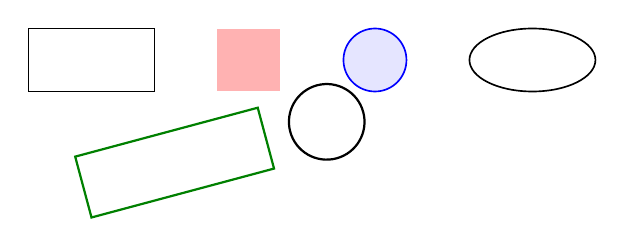
\begin{tikzpicture}[scale=0.8]
\draw (0,0) rectangle (2,1);
\fill[red!30] (3,0) rectangle +(1,1);
\filldraw[box] (5.5,0.5) circle (0.5);
\draw (8,0.5) ellipse (1 and 0.5);
\begin{scope}[xshift=1cm,yshift=-2cm,rotate=15,thick]
  \draw[green!50!black] (0,0) rectangle (3,1);
  \draw (4,0.5) circle[radius=6mm];
\end{scope}
\end{tikzpicture}
\end{center}
After the picture, a last paragraph.
\end{document}
